% !TEX encoding = UTF-8
% !TEX TS-program = pdflatex
% !TEX root = ../arsclassica.tex
% !TEX spellcheck = it-IT

%************************************************
\chapter{Strumenti per la creazione di dataset}
\label{cap:tsis-sensors}
%************************************************
Al fine di valutare le prestazioni degli algoritmi di apprendimento e classificazione delle \acl{CTBN} è emersa la necessità di generare dei dataset adeguati a tale scopo.

Come già specificato in precedenza, le \acs{CTBN} sono un modello stocastico dedito alla rappresentazione dell'evoluzione di sistemi dinamici, cioè di fenomeni che evolvono nel tempo, rappresentati come insiemi di traiettorie multi-variate. Si è quindi scelto di generare dei dataset che rappresentassero un tipico sistema dinamico complesso: il traffico automobilistico su rete urbana.

Tale scelta non è finalizzata al mero esercizio delle tecniche di apprendimento e classificazione descritte e sviluppate, bensì è motivata dalla necessità di individuare delle possibili strategie di ottimizzazione del problema del traffico.

Infatti, il traffico intenso è un problema che affligge tutte le grandi città quotidianamente. La congestione delle reti urbane incide negativamente sulla qualità della vita. Il tempo perso in coda dagli automobilisti ha ripercussioni in primis sulle attività economiche: alcuni studi a riguardo stimano le perdite del sistema economico italiano da esso derivanti in $6,4$ \acsfont{MLD} di \euro{} annui (citazione Bocconi). A ciò si aggiunga l'impatto negativo del traffico sull'ambiente e quindi sulla salute: l'aumento dei tassi di diossina nell'aria è correlato all'aumento delle malattie respiratorie (\eg{} asma) e immunitarie (\eg{} allergie), o peggio all'insorgenza di tumori (citazioni 2 e 3). Inoltre, elevati livelli di traffico sono fonte di stress da cui possono derivare ulteriori complicazioni. Le problematiche citate evidenziano i costi ingenti che il problema del traffico impone alla collettività. Ne deriva la necessità di affrontare tale problema per cercare di ridurne l'impatto negativo. Tra gli approcci finalizzati al miglioramento delle condizioni del traffico urbano emerge, per il grande impatto atteso in termini di benefici, l'ottimizzazione dei piani semaforici in base alle condizioni di traffico. L'ottimizzazione semaforica è un problema complesso, e pochi degli approcci proposti in letteratura (servono citazioni) possono essere effettivamente applicati nella realtà se non con delle grosse semplificazioni, ciò a causa della difficoltà computazionale che li caratterizza. Un modo per risolvere questo problema, non nuovo alla letteratura (serve citazione), è semplificare il problema dividendolo in due step:
\begin{itemize}
    \item classificazione del profilo di traffico
    \item selezione del piano semaforico ad esso associato.
\end{itemize}
In questa tesi affrontiamo il primo passo: la classificazione dei profili di traffico, propedeutico all'ottimizzazione del problema descritto. Inoltre, l'algoritmo di apprendimento strutturale, descritto nel capito \vref{cap:structurallearning}, fornisce la mappa delle relazioni nel tempo tra i vari sensori della rete stradale; ciò si traduce in uno strumento di controllo e osservazione della stessa.

Con l'ausilio di un software commerciale, \acf{TSIS} (versione $\geq$ 6.2) e di una sua \acl{RTE} appositamente sviluppata al fine di monitorare e tracciare il passaggio dei veicoli, sono stati generati dei dataset contenenti un insieme di documenti rappresentanti la presenza (durante l'evolvere del tempo) di veicoli sui sensori di una rete stradale.

In questo capitolo si presentano sia i succitati strumenti utilizzati per la creazione di reti stradali e relativi modelli di simulazione, sia lo strumento ideato per la creazione di dataset relativi al traffico.

Relativamente, invece, al processo pratico di creazione dei dataset si rimanda alla~\autoref{sec:create-dataset-howto}.

\section{TSIS}
\label{sec:tsis}
\acf{TSIS} è un \acl{IDE}\footnote{Un \acl{IDE}, comunemente chiamato anche \ACF{IDE}, è un insieme di programmi finalizzati a supportare il processo di sviluppo dei software. Generalmente, un \acs{IDE} è costituito da uno strumento per la creazione e modifica del codice sorgente, un compilatore o un interprete, strumenti per l'automazione dello sviluppo e la qualità del codice sorgente.}, distribuito commercialmente da McTrans\footnote{McTrans Moving Technology: \url{http://mctrans.ce.ufl.edu}.} e supportato dalla \acf{FWHA}\footnote{Agenzia del Dipartimento dei Trasporti degli Stati Uniti d'America: \\ \url{www.fhwa.dot.gov}.}, il cui scopo ultimo è permettere la simulazione e l'analisi di modelli di reti stradali.

\acs{TSIS} è costituito da insieme di strumenti dedicati alla creazione di reti stradali e relativi modelli di simulazione, all'esecuzione, e eventualmente alla visualizzazione, di tali modelli, così come all'interpretazione dei risultati ottenuti. Tale insieme di strumenti è reso accessibile tramite delle interfaccie grafiche\footnote{Un'interfaccia grafica, nota anche come \acf{GUI}, è un tipo di interfaccia utente il cui fine è permettere all'utente di interagire con il software manipolando oggetti grafici convenzionali.}.

L'architettura modulare con cui \acs{TSIS} è realizzato permette, in caso di necessità, di estendere tale ambiente creando degli ulteriori strumenti.

Di seguito si introducono brevemente i concetti relativi a \acs{TSIS} utilizzati nel prosieguo di questo lavoro di tesi.

Tuttavia si osservi che, poiché lo scopo di questa sezione non consiste nel documentare \acs{TSIS}, la sua trattazione esaustiva (\eg{} semantica e lista completa dei tipi di dati rappresentabili) è omessa. A tale fine si rimanda invece alla documentazione ufficiale del software in questione.

\begin{definizione}[Progetto \acs{TSIS}]\label{defn:tsis-proj}
Un progetto \acs{TSIS} è un insieme di modelli di simulazione per una specifica rete stradale.
\end{definizione}

\begin{definizione}[Modello di simulazione \acs{TSIS}]\label{defn:tsis-sim-model}
Un modello di simulazione è costituito da un input (\eg{} variazioni dei flussi di ingresso nella rete, variazioni delle percentuali di svolta dei veicoli nelle intersezioni) per la simulazione di una determinata rete stradale e tutti i dati generati dalla sua esecuzione (\ie{} simulazione).
\end{definizione}
\begin{osservazione}
Un modello di simulazione può anche prevedere che la sua esecuzione sia eseguita più volte. Finché il seme dei numeri casuali non è modificato, esso è sempre considerato un singolo modello di simulazione.
\end{osservazione}

\begin{definizione}[Formato \acs{TRF}]\label{defn:trf-format}
\acs{TRF}\footnote{\acf{TRF}.} è il formato dei file accettati dal simulatore di \acs{TSIS}. Esso codifica e rappresenta una rete stradale e il relativo modello di simulazione specificandone i vari componenti tramite l'utilizzo dei rispettivi \acs{RT} (si veda la~\vref{defn:tsis-rt}).
\end{definizione}
\begin{osservazione}
Il formato \acs{TRF} è equivalente al formato \acs{TRAF}\footnote{\acf{TRAF}.}.
\end{osservazione}

\begin{definizione}[Formato \acs{TNO}]\label{defn:tno-format}
\acs{TNO}\footnote{\acf{TNO}.} è il formato nativo con cui vengono rappresentate in memoria le reti stradali create visivamente tramite l'interfaccia grafica \acs{TRAFED}.
\end{definizione}

\begin{definizione}[\acl{RT}]\label{defn:tsis-rt}
Un \acf{RT} rappresenta il blocco informativo minimo su cui è costruita una rete stradale e il suo modello di simulazione. Nel concreto esso consiste in una singola riga di testo nei file \acs{TRF} contenente un codice identificativo numerico e dei valori per i rispettivi campi accettati nell'ordine prestabilito. Allo stesso modo, tale formato descrive anche il modello di simulazione della rete stradale.
\end{definizione}

\begin{definizione}[\acs{RTE}]\label{defn:rte}
Una \ACF{RTE}, \acl{RTE}, è un'applicazione in grado di comunicare a tempo d'esecuzione con un'altra applicazione esterna. Una \acs{RTE}, in ambiente \emph{Microsoft Windows}, è solitamente compilata separatamente sotto forma di \acs{DLL}\footnote{Una \acf{DLL} è una libreria software che viene caricata dinamicamente in fase di esecuzione, invece di essere collegata staticamente a un eseguibile in fase di compilazione. Queste librerie sono anche chiamate \ACF{DLL}. L'acronimo \acs{DLL} corrisponde all'estensione che tali oggetti hanno in ambiente \emph{Microsoft Windows}. Tuttavia esse sono spesso chiamate più genericamente con il termine librerie condivise (da \emph{shared library}). Nei sistemi \emph{Linux}, esse sono anche note come oggetti \emph{shared object}.} e deve rispettare una determinata interfaccia: deve perciò implementare e esportare determinate funzioni che l'applicazione oggetto della comunicazione chiama a tempo d'esecuzione. Per la comunicazione in ingresso, invece, una \acs{RTE} deve essere collegata alle librerie dell'applicazione con cui intende interfacciarsi, avendo così accesso alle strutture dati e alle funzioni che questa esporta.
\end{definizione}

\subsection{Componenti}\label{subsec:tsis-components}
In questa sezione si elencano gli strumenti che costituiscono l'ambiente di sviluppo \acs{TSIS}.

\begin{description}
\item[CORSIM] \hfill \\
\acs{CORSIM}\footnote{\acf{CORSIM}.} costituisce il componente principale dell'insieme di strumenti denominato \acs{TSIS}. È un simulatore il cui obiettivo è permettere la creazione e l'esecuzione di modelli di simulazione \acs{TSIS}. È composto da due simulatori integrati che rappresentano l'intero sistema di traffico come funzione del tempo: \acs{NETSIM}\footnote{\acf{NETSIM}.} e \acs{FREESIM}\footnote{\acf{FREESIM}.}. Tali simulatori integrati rappresentano, rispettivamente, il traffico sulle strade urbane e non. La simulazione effettuata da tali strumenti è di tipo microscopico: essi modellano individualmente il comportamento di ogni singolo veicolo, prendendo in considerazione per ognuno di essi una serie di variabili, anche di tipo stocastico (\eg{} tipologia di guidatore). Per tale motivo \acs{CORSIM} è dotato di molte possibili opzioni di configurazione e permette lo studio di modelli molto complessi e dettagliati.
\item[TRAFED] \hfill \\
\acs{TRAFED}\footnote{\acf{TRAFED}.} è una \acs{GUI} il cui scopo è permettere la creazione e la modifica di reti stradali e di modelli di simulazione per \acs{CORSIM}.
\item[TShell] \hfill \\
\acs{TShell}\footnote{\acf{TShell}.} è la \acs{GUI} di \acs{TSIS}. Funge da contenitore degli strumenti (preconfigurati, o creati dall'utente) di questo ambiente di sviluppo integrato e permette la gestione dei progetti \acs{TSIS}.
\item[TRAFVU] \hfill \\
\acs{TRAFVU}\footnote{\acf{TRAFVU}.} è una \acs{GUI} finalizzata alla visualizzazione dei modelli di simulazione simulati con \acs{CORSIM}. Essa permette sia di visualizzare in modo animato l'evoluzione del traffico nella rete stradale con una qualsiasi granularità temporale, sia di visualizzare una serie di misure di interesse relative alla simulazione.
\item[TSIS Text Editor] \hfill \\
\acs{TSIS} \acsfont{Text Editor} è uno strumento il cui scopo è facilitare la modifica manuale dei file \acs{TRF}. A tale scopo esso visualizza per ogni \acs{RT} che si intende modificare sia la sua descrizione sia l'insieme dei campi supportati.
\item[TSIS Script Tool] \hfill \\
\acs{TSIS} \acsfont{Script Tool} è uno strumento per la creazione, la modifica e l'esecuzione di codice \acs{VBScript}\footnote{\acf{VBScript} è un linguaggio interpretato, sottoinsieme del linguaggio \emph{Visual Basic}, utilizzato come sostituto o integrazione della linea di comando o per il controllo di applicazioni esterne in ambiente \emph{Microsoft Windows}.}. Questo strumento fornisce un meccanismo utile ad automatizzare le funzionalità di simulazione di \acs{TSIS} (\eg{} esecuzioni multiple dello stesso modello di simulazione variando il seme dei numeri casuali che governa la distribuzione di ingresso dei veicoli nella rete stradale).
\item[TSIS Translator] \hfill \\
\acs{TSIS} \acsfont{Translator} è uno strumento utile alla conversione dei file dal formato \acs{TRF} al formato \acs{TNO} e viceversa. Tale operazione risulta utile al fine di rendere i file \acs{TRF} utilizzabili tramite lo strumento \acs{TRAFED} così come per rendere i file \acs{TNO} utilizzabili con \acs{CORSIM}.
\item[TSIS Output Processor] \hfill \\
\acs{TSIS} \acsfont{Output Processor} è uno strumento finalizzato alla raccolta e l'aggregazione dei dati da \acs{CORSIM} durante l'esecuzione multipla di modelli di simulazione. La sua caratteristica principale consiste nella computazione automatica di un insieme di statistiche predefinite. Esso permette di scegliere sia le statistiche di interesse sia la granularità temporale della loro computazione.
\end{description}

\subsection{Caratteristiche}\label{subsec:tsis-features}
Segue una panoramica il cui scopo è presentare sia le principali capacità, sia i vincoli di modellazione, simulazione e analisi di \acs{TSIS}.

\acs{TSIS}, tramite \acs{CORSIM}, permette la modellazione di reti stradali con le seguenti caratteristiche:

\begin{itemize}
    \item reti stradali urbane, non urbane o miste
    \item controllo quantitativo (\ie{} quantità di veicoli per intervallo temporale, distribuita secondo una distribuzione statistica) e qualitativo (\ie{} tipo di veicoli) dei flussi di veicoli in ingresso nella rete stradale
    \item controllo completo del flusso di traffico (\ie{} percentuali di svolta dei veicoli variabile nel tempo)
    \item supporto per strade con più corsie (massimo $9$)
    \item supporto dei segnali stradali
    \item supporto per gli attraversamenti pedonali
    \item intersezioni non controllate
    \item intersezioni controllate da semafori
    \item canalizzazione delle corsie
    \item piani semaforici predefiniti, dinamici (\eg{} priorità ai veicoli di emergenza) o guidati da algoritmi (\eg{} attivazione del semaforo in base alle rilevazioni effettuate dai sensori)
    \item sensori per la rilevazione del passaggio o della presenza di veicoli
    \item supporto per i mezzi di trasporto pubblico (\ie{} autobus, taxi)
    \item rilevamento di incidenti
    \item supporto per i sistemi di guida anglosassoni
    \item simulazione guidata all'analisi delle code
    \item simulazione guidata allo studio del grado di occupazione della rete stradale
    \item output di dati di interesse aggregati
    \item output di dati statistici collezionati
\end{itemize}

Poiché un modello di simulazione del traffico è caratterizzato dal cambiamento di un insieme di condizioni (\eg{} volumi di traffico, canalizzazione delle corsie, percentuali di svolta dei veicoli) della rete stradale, esso deve specificare, oltre alla natura stessa dei cambiamenti, anche i fattori in base a cui essi avvengono. Il fattore primario che viene preso in considerazione è il tempo. Ne consegue perciò che un modello di simulazione del traffico deve specificare l'intervallo temporale in cui specifici cambiamenti di determinate condizioni avvengono.

\acs{CORSIM} affronta questo problema permettendo di partizionare il tempo totale di simulazione in una serie di periodi temporali (\ie{} \emph{time period}) di durata variabile. Ogni periodo temporale possiede perciò un insieme di dati di input che non variano per tutta la sua durata. Inoltre, i periodi temporali sono a loro volta suddivisi in intervalli temporali (\ie{} \emph{time interval}), anch'essi suddivisi in passi temporali (\ie{} \emph{time step}).

Le principali limitazioni di \acs{TSIS} derivano dalle modalità con cui \acs{CORSIM} implementa la gestione del tempo: la lista dei periodi temporali è rappresentata internamente tramite un array statico di dimensione prefissata. Nello specifico, un modello \acs{CORSIM} può essere costituito da un massimo di $19$ periodi temporali, ognuno dei quali viene specificato tramite il \acs{RT} $03$, e può avere una durata compresa tra i $10$ e i $9999$ secondi. Ognuno di tali periodi temporali è suddiviso in intervalli (specificati tramite dei \acs{RT} $04$) la cui durata, compresa tra $1$ e $200$ secondi, deve essere un sottomultiplo della durata del periodo temporale cui appartiene. Infine, ogni intervallo temporale è partizionato in passi temporali: \acs{NETSIM} utilizza un passo temporale fisso di $1$ secondo mentre \acs{FREESIM} opera in base al passo temporale specificato dall'utente. Poiché i due modelli di simulazione microscopica che costituiscono \acs{CORSIM} operano in modo sincronizzato, la durata del passo temporale di \acs{FREESIM}, anche se compresa nell'intervallo $[0.1,1]$ secondi, non può essere specificata liberamente dall'utente. All'utente è permesso specificare solo il numero di passi temporali di \acs{FREESIM} (tramite il campo $1$, \acs{RT} $04$) che devono essere eseguiti per ogni secondo di simulazione. Tale approccio permette perciò di utilizzare dei passi temporali di durata minore per il simulatore \acs{FREESIM} mantenendo la sincronizzazione con il simulatore \acs{NETSIM}. La~\vref{tab:fresim-time-steps} mostra la corrispondenza tra il numero di passi temporali di \acs{FREESIM} e la reale durata che verrà loro assegnata.

\begin{table}[h]%
\centering%
\begin{tabular}{+c^c}
\toprule\rowstyle{\bfseries}%
Valore del campo $1$    & Durata del passo temporale in \acs{FREESIM}   \\
                        & (sec)                                         \\\otoprule%
1                       & 1.0                                           \\
2                       & 0.5                                           \\
3                       & 0.333333                                      \\
4                       & 0.25                                          \\
5                       & 0.2                                           \\
6                       & 0.166667                                      \\
7                       & 0.142857                                      \\
8                       & 0.125                                         \\
9                       & 0.111111                                      \\
10                      & 0.1                                           \\\bottomrule
\end{tabular}
\caption[Durata dei passi temporali in \acs{FREESIM}]{Relazione tra numero di passi temporali per ogni secondo di simulazione e durata effettiva del passo temporale in \acs{FREESIM}.}
\label{tab:fresim-time-steps}
\end{table}

La~\vref{fig:corsim-time} mostra, tramite un esempio, quanto appena descritto relativamente alla rappresentazione del tempo in \acs{CORSIM}.

Si osservi, inoltre, che la granularità temporale massima con cui è possibile ottenere statistiche cumulative, e, in generale, dati relativi alla simulazione, corrisponde alla durata scelta per gli intervalli temporali (si veda a tal riguarda la documentazione relativa al tipo \acs{RT} $05$). Si consideri ad esempio la~\vref{fig:corsim-time}: in tal caso non sarà possibile ottenere dati cumulati relativi a un intervallo di tempo minore di $60$ secondi.

\begin{figure}[ht]
\centering
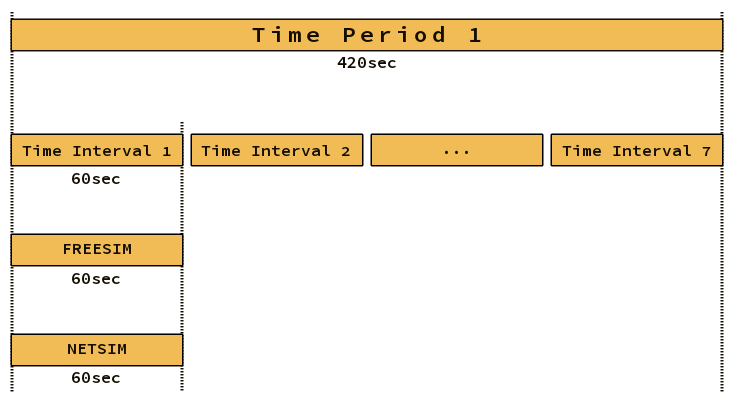
\includegraphics[width=1\columnwidth]{corsim-time}
\caption[Gestione del tempo in \acs{CORSIM}]{Esempio di suddivisione gerarchica delle unità temporali in \acs{CORSIM}. Un \emph{time period} della durata di $420$ secondi è suddiviso in $7$ \emph{time interval}, ciascuno della durata di $60$ secondi. Ogni \emph{time interval} verrà poi automaticamente diviso in $60$ \emph{time step} da $1$ secondo ciascuno per \acs{NETSIM} (\ie{} linee rosse). La durata di tali \emph{time step} di \acs{NETSIM} può o meno coincidere, come accade in questo esempio, con quella assegnata ai \emph{time step} di \acs{FREESIM} a seconda del valore del campo $1$ del \acs{RT} $04$ nel modello \acs{CORSIM}.}
\label{fig:corsim-time}
\end{figure}

La gestione del tempo che \acs{CORSIM} attua implica quindi alcune limitazioni:
\begin{itemize}
    \item il tempo massimo di simulazione, benché sufficiente nella maggior parte dei casi, è di circa $52$ ore
    \item la massima granularità con cui è possibile raccogliere informazioni è di $1$ secondo, impostando a tale valore la durata degli intervalli temporali
    \item i dati raccolti dalla simulazione sono sempre aggregati in base alla durata dell'intervallo temporale cui si riferiscono.
\end{itemize}
Tali vincoli rendono impossibile recuperare l'output dei sensori a tempo continuo in modo non aggregato o in generale con una granularità temporale inferiore a $1$ secondo. Al fine di sorpassare tali limitazioni si è proceduto sviluppando una \acl{RTE} apposita, \acsfont{Sensors} \acs{DLL}, descritta dettagliatamente nella \vref{sec:sensors-rte}. Al fine di rendere la descrizione di tale software maggiormente chiara, è necessario presentare il meccanismo di estensione di \acs{CORSIM}. La sezione che segue affronta questo argomento.

\section{Creazione di estensioni TSIS}
\acs{TSIS} espone un meccanismo finalizzato all'estensione delle sue funzionalità tramite la creazione, da parte dell'utente, di altri strumenti da integrare nell'ambiente di sviluppo. Tali strumenti, interfacciandosi direttamente con \acs{CORSIM}, possono modificarne o aumentarne la logica di simulazione, collezionare dati o monitorare eventi speciali (\eg{} indicenti).

In questa sottosezione si presenta il funzionamento dei meccanismi di interfacciamento (\ie{} più brevemente detti \acs{API}\footnote{Con il termine
\acf{API} si indica un insieme di procedure rese disponibili all'esterno, di solito raggruppate a formare un insieme di strumenti specifici per l'espletamento di un determinato compito all'interno di un programma.}) tra \acs{CORSIM} e strumenti esterni, a cui ci si riferirà da questo momento in poi con il termine \acs{CORSIM} \acs{RTE}.

\subsection{Requisiti}
Al fine di sviluppare e compilare con successo una \acs{CORSIM} \acs{RTE} in \CC{} è necessario disporre dei seguenti strumenti:
\begin{itemize}
    \item il compilatore della piattaforma \emph{Microsoft Visual \CC{}}
    \item il pacchetto software di \acs{TSIS}, il quale include di default tutti i componenti necessari mostrati dalla~\vref{fig:tsis-corsim-arch} (ad eccezione, chiaramente, del componente \acs{RTE}).
\end{itemize}
Si osservi, inoltre, che è possibile sviluppare una \acs{CORSIM} \acs{RTE} anche in linguaggio \lstinline[]|C| o \lstinline[]|FORTRAN|.

\subsection{Architettura di CORSIM}

La~\vref{fig:tsis-corsim-arch} illustra l'architettura modulare di \acs{CORSIM} e il suo funzionamento all'interno dell'ambiente di sviluppo \acs{TSIS}.
\begin{figure}
\centering
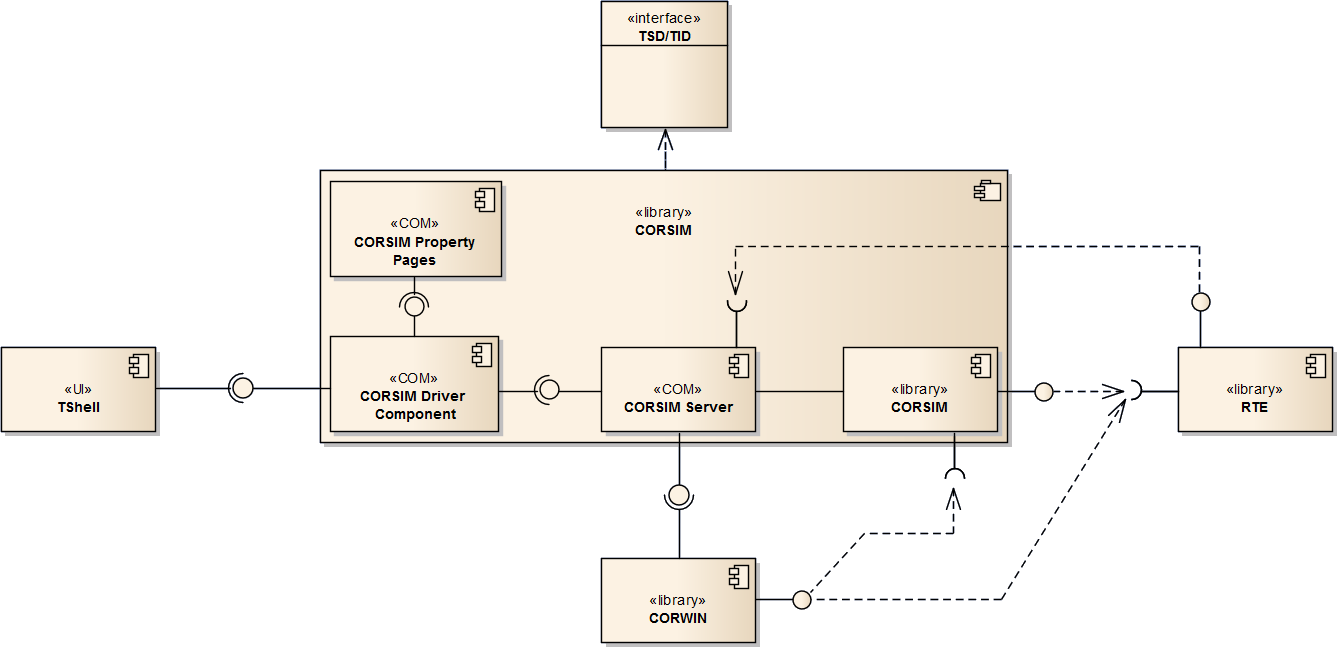
\includegraphics[width=0.925\columnwidth]{tsis-corsim-components}
\caption[Diagramma dei componenti di \acs{CORSIM}]{Porzione del diagramma dei componenti di \acs{TSIS}: mostra l'architettura modulare e il funzionamento di \acs{CORSIM} all'interno di \acs{TSIS}.}
\label{fig:tsis-corsim-arch}
\end{figure}
Si osservi che i componenti che costituiscono \acs{CORSIM} sono di due tipi: librerie \acs{DLL} e moduli \acs{COM}\footnote{Il \acf{COM} è uno standard per componenti software ideato da \emph{Microsoft}. Il suo fine consiste nel permettere la comunicazione fra processi e la creazione dinamica di oggetti. Una interfaccia \acs{COM} è una collezione di funzioni, incapsulata in un componente software binario e neutrale rispetto al linguaggio.}. Il \acs{CORSIM} \acsfont{Driver Component}, ad esempio, è il modulo \acs{COM} di \acs{TSIS} preposto a interfacciare \acs{CORSIM} e \acs{TShell}, permettendo così il controllo e l'esecuzione di \acs{CORSIM}, delle \acs{RTE} create dall'utente e degli altri strumenti (\eg{} \acs{TSIS} \acsfont{Output Processor}) di \acs{TSIS} tramite \acs{GUI}.

Anche se la~\vref{fig:tsis-corsim-arch} mostra per completezza l'intera architettura di \acs{CORSIM}, si procede con la descrizione delle interfacce di \acs{CORSIM} preposte alla comunicazione con \acs{RTE} sviluppate dall'utente, identificate dalle frecce tratteggiate e numerate.

Per ogni passo temporale di simulazione, il \acs{CORSIM} \acsfont{Server} chiama una serie di funzioni di \acs{CORSIM} finalizzate a guidare l'andamento della simulazione. Quando una \acs{RTE} viene inserita nell'ambiente di sviluppo integrato, il \acs{CORSIM} \acsfont{Server} chiama anche le funzioni che la \acs{RTE} esporta in base ai messaggi che riceve da \acs{CORSIM} durante la sua esecuzione. Questa interfaccia è rappresentata dalla freccia $1$ nella~\vref{fig:tsis-corsim-arch}; la~\autoref{subsec:corsim-lifecycle} \vpageref{subsec:corsim-lifecycle} riporta maggiori dettagli sui punti di chiamata che \acs{CORSIM} espone.

\acs{TSIS} fornisce inoltre una \acs{API}, identificata dalla freccia $2$ nella~\vref{fig:tsis-corsim-arch}, chiamata \acsfont{CORWIN}, che permette alle \acs{RTE} di inviare messaggi al modulo \acs{CORSIM} \acsfont{Server} affinché essi siano visualizzati in \acs{TShell} dal \acs{CORSIM} \acsfont{Driver Component}.

Infine, una \acs{RTE} può accedere direttamente a una serie di funzioni e strutture dati esportate da \acs{CORSIM} nella memoria condivisa. Anche se non è possibile riferirsi a questo meccanismo di comunicazione come una \acs{API} vera e propria, nel prosieguo, ci riferiremo ad essa con il termine \acs{CORSIM} \acs{API} al fine di semplificare la discussione. Perciò, la \acs{CORSIM} \acs{API}, rappresentata dalla freccia $3$ della~\vref{fig:tsis-corsim-arch}, oltre a permettere l'estrazione di informazioni relative alla simulazione, permette alla \acs{RTE} di controllare, eventualmente, molti aspetti della simulazione operata da \acs{CORSIM} (\eg{} aborto della simulazione).

Si osservi che, anche se la~\vref{fig:tsis-corsim-arch} non evidenzia tale possibilità, l'architettura di \acs{CORSIM} supporta l'utilizzo di più \acs{RTE} contemporaneamente.

\begin{nota}
Un attento osservatore noterà come \acs{CORSIM}, la libreria finalizzata al processo di simulazione, sia a sua volta una \acs{RTE} automaticamente collegata ai moduli \acs{CORSIM} \acsfont{Server} e \acsfont{CORWIN}. Inoltre, la~\vref{fig:tshell-tool-config-1} fa notare come tutti i componenti (elencati e descritti nella~\autoref{subsec:tsis-components} \vpageref{subsec:tsis-components}) dell'ambiente di sviluppo \acs{TSIS} siano anch'essi dei moduli architetturalmente uguali alle \acs{RTE}.
\end{nota}

\subsection{Ciclo di vita di CORSIM}\label{subsec:corsim-lifecycle}
Di seguito si presenta il ciclo di vita di \acs{CORSIM} descrivendo i punti di chiamata che esso esporta tramite apposite funzioni affinché una \acs{RTE}, implementando ed esportando una funzione per almeno uno di essi, possa interfacciarsi con il processo di simulazione. Tali informazioni sono quindi relative alla \acs{API} rappresentata dalla freccia $1$ nella~\vref{fig:tsis-corsim-arch}. Le modalità di implementazione e utilizzo in \CC{} di tale \acs{API} sono illustrate nella~\autoref{subsec:tsis-api-examples} \vpageref{subsec:tsis-api-examples}.

La~\vref{tab:corsim-lifecycle} descrive tutti i punti di chiamata relativi alla linea di esecuzione temporale di \acs{CORSIM}.
\begin{table}[ht]%
\begin{tabularx}{\columnwidth}{+l^X}
\toprule\rowstyle{\bfseries}%
Punto di chiamata                   & Descrizione                                   \\
\otoprule%
\lstinline[]|Initialize|            & \small Chiamato all'inizio della simulazione prima della fase di inizializzazione \acs{CORSIM} ma dopo la lettura del file \acs{TRF} di input.                                                            \\
\lstinline[]|PostVehicleEmit|       & \small Chiamato ad ogni \emph{time step} dopo che i veicoli sono stati immessi nella rete stradale.                                                                           \\
\lstinline[]|PreNetsimVehicle|      & \small Chiamato ad ogni \emph{time step} appena prima che i veicoli inizino a muoversi nel sotto-modello \acs{NETSIM}.                                                                                   \\
\lstinline[]|PreNetsimSignal|       & \small Chiamato ad ogni \emph{time step} appena prima che i segnali (\eg{} semafori) del sotto-modello \acs{NETSIM} vengano impostati.                                                                  \\
\lstinline[]|PostNetsimTimestep|    & \small Chiamato in corrispondenza della fine del processo di simulazione di ogni \emph{time step} di \acs{NETSIM} e prima che \acs{FREESIM} inizi a simulare il suo relativo sotto-modello.                   \\
\lstinline[]|PreFresimVehicle|      & \small Chiamato ad ogni \emph{time step} appena prima che i veicoli inizino a muoversi nel sotto-modello \acs{FREESIM}.                                                                                   \\
\lstinline[]|PreFresimSignal|       & \small Chiamato ad ogni \emph{time step} appena prima che i segnali (\eg{} semafori) del sotto-modello \acs{FREESIM} vengano impostati.                                                                  \\
\lstinline[]|PostFresimTimestep|    & \small Chiamato in corrispondenza della fine del processo di simulazione di ogni \emph{time step} di \acs{FREESIM}.
                                                                                    \\
\lstinline[]|BeginSimulation|       & \small Chiamato dopo l'inizializzazione di \acs{CORSIM} (\ie{} rete stradale piena) in corrispondenza dell'inizio della simulazione.                                                                        \\
\lstinline[]|TimeStepComplete|      & \small Chiamato in corrispondenza della fine del processo di simulazione di ogni \emph{time step}.                                                                                   \\
\lstinline[]|TimeIntervalComplete|  & \small Chiamato in corrispondenza della fine del processo di simulazione di ogni \emph{time interval}.                                                                                   \\
\lstinline[]|TimePeriodComplete|    & \small Chiamato in corrispondenza della fine del processo di simulazione di ogni \emph{time period}.                                                                                   \\
\lstinline[]|TimePeriodValidated|   & \small Chiamato in corrispondenza della fine del processo di lettura e validazione del file di input relativo a ogni \emph{time period}, prima dell'inizializzazione e dell'effettivo inizio del processo di simulazione di ogni \emph{time period}.                                                                                   \\
\lstinline[]|SimulationComplete|    & \small Chiamato in corrispondenza della fine della simulazione e prima della completa terminazione del processo.                                                                           \\
\lstinline[]|Shutdown|              & \small Chiamato appena prima che l'esecuzione di \acs{CORSIM} termini.
                                                                                    \\
\lstinline[]|Exit|                  & \small Chiamato in corrispondenza della fine dell'intero processo di simulazione.
                                                                                    \\\bottomrule
\end{tabularx}
\caption[Ciclo di vita di \acs{CORSIM}]{Descrizione di punti di chiamata che \acs{CORSIM} espone all'esterno.}
\label{tab:corsim-lifecycle}
\end{table}
Una volta compilata la \acs{RTE} e ottenuto il relativo file \acs{DLL}, ognuno dei punti di chiamata di \acs{CORSIM} deve essere associato alla rispettiva funzione implementata dalla \acs{RTE}. La~\autoref{subsec:rte-corsim-linking} \vpageref{subsec:rte-corsim-linking} descrive in maggior dettaglio tale processo.

\subsection{Collegare una RTE a CORSIM}\label{subsec:rte-corsim-linking}
Questa sottosezione illustra i passi necessari a espletare il processo di collegamento (\ie{} \emph{linking}) di una \acs{RTE} a \acs{CORSIM}. Tale processo è eseguibile direttamente tramite \acs{TShell}.

A scopo esemplificativo si descrive come aggiungere la \acs{RTE} per il rilevamento e tracciamento del passaggio dei veicoli sui sensori (descritta nella~\vref{sec:sensors-rte}). Tale operazione viene svolta tramite il menù \emph{Tools} di \acs{TShell} scegliendo la voce \emph{Tool Configuration} e cliccando sul pulsante per l'aggiunta (\ie{} \emph{Add}) di una \acs{RTE}. La~\vref{fig:tshell-tool-config-1} mostra lo strumento di configurazione degli strumenti appartenenti all'ambiente di \acs{TSIS}.

\begin{figure}[H]
\centering
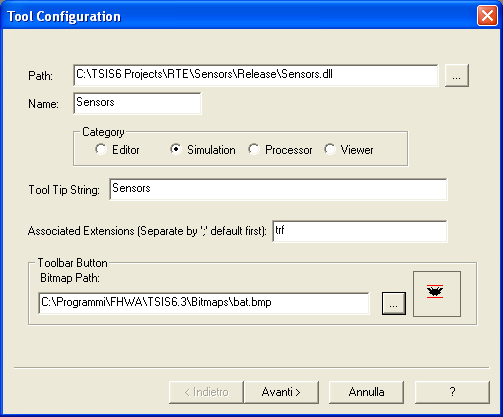
\includegraphics[width=1\columnwidth]{tshell-tool-config-1}
\caption[Aggiunta di una \acs{RTE} a \acs{TSIS}]{Strumento finalizzato all'aggiunta di una \acs{RTE} a \acs{TSIS}.}
\label{fig:tshell-tool-config-1}
\end{figure}
Specificato il percorso a cui risiede il file \acs{DLL} della \acs{RTE}, il tipo di \acs{RTE}, il nome e l'icona che si intende assegnare a tale strumento e il tipo di file a cui va associato (\eg{} \acs{TRF}), la \acs{RTE} è aggiunta a \acs{TSIS}. La~\vref{fig:tshell-toolbar} mostra la barra degli strumenti di \acs{TShell} quando un file \acs{TRF} viene aperto: essa contiene il pulsante per l'avvio della \acs{RTE} appena aggiunta all'ambiente di sviluppo \acs{TSIS}.
\begin{figure}[H]
\centering
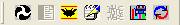
\includegraphics[width=0.4\columnwidth]{tshell-toolbar}
\caption[Barra degli strumenti di \acs{TShell}]{Barra degli strumenti di \acs{TShell} contenente il pulsante per l'invocazione della \acs{RTE} aggiunta all'ambiente di sviluppo \acs{TSIS}.}
\label{fig:tshell-toolbar}
\end{figure}

Tuttavia, come detto, le funzioni della \acs{RTE} devono essere collegate ai punti di chiamata di \acs{CORSIM} affinché la \acs{RTE} risulti completamente funzionante. Per adempiere tale operazione è necessario utilizzare nuovamente lo strumento di configurazione cliccando sul pulsante per la modifica (\ie{} \emph{Edit}) di una \acs{RTE}. A questo punto, selezionando la scheda relativa alle \acs{RTE}, è possibile invocare lo strumento per effettuare il succitato collegamento. La~\vref{fig:tshell-tool-config-8} mostra il processo di collegamento tra le funzioni della \acs{RTE} e i punti di chiamata di \acs{CORSIM}.
\begin{figure}[H]
\centering
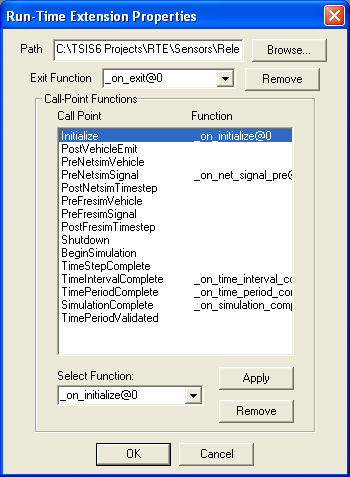
\includegraphics[width=0.8\columnwidth]{tshell-tool-config-8}
\caption[Collegamento delle funzioni della \acs{RTE} a \acs{CORSIM}]{Collegamento delle funzioni della \acs{RTE} ai rispettivi punti di chiamata di \acs{CORSIM}.}
\label{fig:tshell-tool-config-8}
\end{figure}

Inoltre, può essere necessario dover configurare la \acs{RTE} aggiunta in base alle sue esigenze, così come modificare alcune funzionalità di \acs{CORSIM} relativamente ad essa. Ad esempio, la \acs{RTE} per il monitoraggio e il tracciamento del passaggio dei veicoli sui sensori non necessita che i file di output di \acs{CORSIM} vengano generati, né che vengano generati i file per la visualizzazione animata della simulazione in \acs{TRAFED}. Inoltre, tale \acs{RTE}, non necessita che la simulazione \acs{CORSIM} sia eseguita più volte. La~\vref{fig:tshell-tool-config-35} mostra la configurazione di tali opzioni.
\begin{figure}[H]
\centering
\subfloat[Proprietà di \acs{CORSIM}.]
{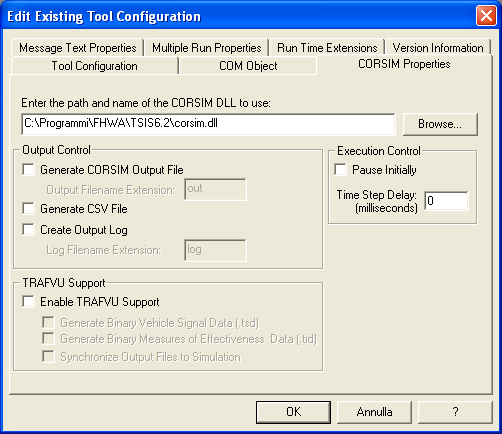
\includegraphics[width=0.8\columnwidth]{tshell-tool-config-3}} \\
\subfloat[Impostazioni proprietà d'esecuzione di \acs{CORSIM}.]
{\label{fig:ipsum}%
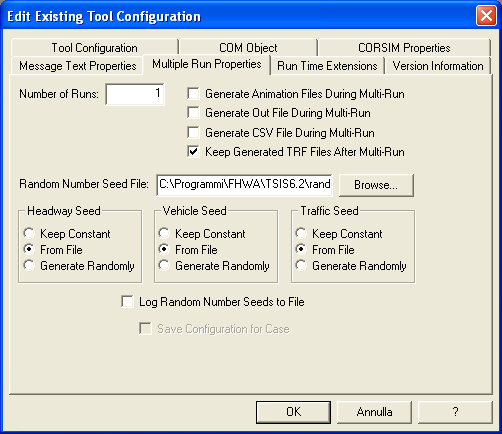
\includegraphics[width=0.8\columnwidth]{tshell-tool-config-5}}
\caption[Configurazione delle proprietà di \acs{CORSIM}]{Configurazione delle proprietà di \acs{CORSIM} per la \acs{RTE}: disattivazione dell'output di \acs{CORSIM}, della generazione dell'input per \acs{TRAFED} e delle esecuzioni multiple della simulazione.}
\label{fig:tshell-tool-config-35}
\end{figure}

\cleardoublepage
\subsection{Utilizzo delle API}\label{subsec:tsis-api-examples}
Lungi dal volere fornire una documentazione esaustiva delle \acs{API} dell'ambiente di sviluppo \acs{TSIS}, in questa sezione, si intende presentare, tramite esempi, le modalità di utilizzo di tali \acs{API} in linguaggio \CC{}.

Ad esempio, il listato~\ref{lst:callpoint-api} mostra il codice di intestazione necessario a definire ed esportare la funzione \lstinline[]|on_initialize| (listato~\ref{lst:callpoint-impl}), che, come mostrato dalla~\vref{fig:tshell-tool-config-8} viene collegata al punto di chiamata \lstinline[]|Initialize| di \acs{CORSIM}. Si osservi che la scelta del nome di tale funzione non è vincolata ad alcun criterio.

\vspace*{8pt}\lstinputsourcecode[language=cpp, caption=Costrutto per l'esportazione delle funzioni \acs{RTE}, label=lst:callpoint-api]{codes/callpointapi}

\vspace*{8pt}\lstinputsourcecode[language=cpp, caption=Esempio di funzione \acs{RTE} esportata, label=lst:callpoint-impl]{codes/callpointimpl}

Il listato~\ref{lst:corwin-api} illustra invece come importare una delle funzioni esposte dalla \acsfont{CORWIM} \acs{API} in una \acs{RTE}. Nello specifico, l'esempio in questione, è relativo all'importazione della funzione \lstinline[]|OutputString|, finalizzata all'invio di messaggi di output a \acs{TShell} durante la simulazione \acs{CORSIM}.

\vspace*{8pt}\lstinputsourcecode[language=cpp, caption=Importazione delle \acsfont{CORWIN} \acs{API}, label=lst:corwin-api]{codes/corwinapi}

Infine, come già detto, \acs{CORSIM} permette l'accesso alla maggior parte dei dati che esso manipola durante la simulazione, esportandoli nella memoria condivisa. Tali dati sono dei seguenti tipi:
\begin{enumerate}
    \item variabili scalari (non array)
    \item array allocati staticamente
    \item array allocati dinamicamente
    \item funzioni esposte tramite \acs{API}.
\end{enumerate}

Il listato~\ref{lst:corsim-api-dll-import} mostra il costrutto utilizzabile per l'importazione di dati e funzioni dalla cosiddetta \acs{CORSIM} \acs{API}.
\vspace*{8pt}\lstinputsourcecode[language=cpp, caption=Costrutto per l'importazione delle \acs{CORSIM} \acs{API}, label=lst:corsim-api-dll-import]{codes/corsimapidllimport}

Tale costrutto viene poi utilizzato per l'effettiva importazione di dati e funzioni da \acs{CORSIM}. Il listato~\ref{lst:corsim-api} riporta un esempio di importazione per ogni tipo di dati che le \acs{CORSIM} \acs{API} rendono disponibile:
\begin{enumerate}
    \item a~\autoref{lst:netsim-num-dets-import} si importa il numero di sensori presenti sulla rete stradale urbana, esportato da \acs{CORSIM} tramite la variabile scalare \lstinline[]|NETSIM_DETECTORS_mp_NUMDET| e rinominato, a~\autoref{lst:netsim-num-dets-assign}, in \lstinline[]|net_det_num|
    \item a~\autoref{lst:netsim-nmap-import} si importa la lista statica (\ie{} di dimensione massima prefissata) dei numeri identificativi assegnati dall'utente ai nodi della rete stradale, \lstinline[]|SIN075.NMAP|; rinominata a~\autoref{lst:netsim-nmap-assign} in \lstinline[]|net_node_num|
    \item a~\autoref{lst:netsim-dets-mod-import} si importa la lista dinamica delle informazioni sui sensori, \lstinline[]|*NETSIM_DETECTORS_mp_DETMOD|; rinominata, a~\autoref{lst:netsim-dets-mod-assign}, in \lstinline[]|net_det_mod|
    \item a~\autoref{lst:netsim-abort-func-import} si importa \lstinline[]|abortcorsim|, una funzione delle \acs{CORSIM} \acs{API} finalizzata al controllo dell'esecuzione della simulazione da parte della \acs{RTE}
\end{enumerate}

\vspace*{8pt}\lstinputsourcecode[language=cpp, caption=Importazione di oggetti delle \acs{CORSIM} \acs{API}, label=lst:corsim-api]{codes/corsimapi}

\cleardoublepage
\section{Estensione}\label{sec:sensors-rte}
Avendo presentato l'ambiente di sviluppo \acs{TSIS} e le \acs{API} che esso fornisce per la sua estensione, è ora possibile descrivere l'\acl{RTE} sviluppata al fine di generare i succitati dataset.

Come detto nella~\autoref{subsec:tsis-features} \vpageref{subsec:tsis-features}, una delle principali limitazioni di \acs{CORSIM} consiste nell'impossibilità di ottenere dei dati non aggregati dal processo di simulazione. Ciò poiché il minimo intervallo temporale che \acs{CORSIM} permette di utilizzare è pari a $1$ secondo per le reti stradali urbane e al più $0.1$ secondi per le reti stradali extraurbane. Perciò, è emerso il problema di sorpassare tale limitazione. La \acs{RTE} sviluppata, \acsfont{Sensors} \acs{DLL}, risponde a tale necessità monitorando determinati elementi (\ie{} i sensori) di un qualsiasi tipo di rete stradale e tracciando gli eventi ad essi correlati (\ie{} passaggio di un veicolo) su un file di output esterno a \acs{TSIS}. Lo scopo di questa sezione consiste nel presentare il funzionamento di \acsfont{Sensors} \acs{DLL}.

\subsection{Sensors DLL}\label{subsec:sensors-dll}
L'obiettivo ultimo di \acsfont{Sensors} \acs{DLL} consiste nella generazione di un file \acs{CSV}\footnote{\acf{CSV} è un formato basato su file di testo utilizzato per l'importazione ed esportazione (ad esempio da fogli elettronici o database) di una tabella di dati.} che rappresenti il passaggio dei veicoli sui vari sensori presenti nella rete stradale nel tempo. Il monitoraggio dei sensori deve essere effettuato con la massima granularità temporale possibile (\ie{} $0.1$ secondi), anche nel caso di reti stradali urbane.

A tale scopo si è utilizzato il dato \lstinline[]|NETSIM_DETECTORS_mp_DETON|, rinominato in \lstinline[]|net_det_on|, esportato da \acs{CORSIM} nella memoria condivisa. Tale campo indirizza un array dinamico la cui lunghezza è pari al numero di sensori sulla rete stradale. Ognuno degli elementi di tale array è costituito da $10$ bit: l'$i$-esimo bit rappresenta l'attivazione (\ie{} $1$) o meno del relativo sensore nell'$i$-esimo passo temporale minimo (\ie{} $0.1$ secondi). Ogni elemento rappresenta perciò il passaggio dei veicoli sul sensore durante un intervallo temporale fisso di $1$ secondo.

Di seguito si presentano le operazioni principali che \acsfont{Sensors} \acs{DLL} effettua:
\begin{enumerate}
    \item ottenere il nome del file \acs{TRF} di input, rappresentante la rete stradale e il modello di simulazione
    \item effettuare il \emph{parsing}\footnote{Il \emph{parsing} consiste nel processo atto ad analizzare un input in modo da determinare la sua struttura grammaticale grazie ad una data grammatica formale.} di tale file creando gli oggetti relativi a ogni elemento (\eg{} intersezioni, strade, sensori) della rete stradale
    \item rilevare il passaggio dei veicoli sui sensori ogni secondo
    \item ricostruire l'intero flusso di veicoli su ogni sensore durante tutto il tempo di simulazione
    \item creare un file di output che contenga le informazioni ottenute.
\end{enumerate}
Le operazioni $1$ e $2$ vengono compiute in corrispondenza dell'inizializzazione di \acs{CORSIM} e quindi della \acs{RTE}. Il risultato di tali operazioni è un insieme di istanze correlate rappresentanti gli elementi della rete stradale di input e le caratteristiche di ognuno di essi. Il diagramma delle classi di \acsfont{Sensors} \acs{DLL}, mostrato in~\vref{fig:sensors-class-diagram}, illustra le relazioni di associazione e aggregazione degli oggetti con cui si è scelto di rappresentare le reti stradali \acs{TSIS}. La classe \lstinline[]|CNetwork| rappresenta la rete stradale, composta da un insieme di intersezioni e strade, elementi rappresentati rispettivamente dalle classi \lstinline[]|CNode| e \lstinline[]|CLink|. Ogni strada può a sua volta essere composta da più corsie, elementi rappresentati tramite la classe \lstinline[]|CLane|, e contenere dei sensori, elementi rappresentati tramite la classe \lstinline[]|CDetector|. Inoltre, poiché è possibile che alcuni sensori siano posti esclusivamente su una corsia piuttosto che su tutta la superficie della strada, sussiste una relazione anche fra la classe rappresentante le corsie e quella rappresentante i sensori. Invece, la classe \lstinline[]|CBinary| non rappresenta alcun elemento concreto della rete stradale: la sua funzione è esclusivamente quella di incapsulare l'intero \lstinline[]|net_det_on| e convertirlo nella corretta sequenza di bit rappresentante il flusso dei veicoli su un sensore. La procedura che effettua tali operazioni di inizializzazione della rete stradale nella \acs{RTE}, chiamata \lstinline[]|on_initialize|, è collegata al punto di chiamata \lstinline[]|Initialize|, così come mostrato dalla~\vref{fig:tshell-tool-config-8}.

Configurata la rete stradale, \acsfont{Sensors} \acs{DLL} può monitorare i sensori di pari passo con l'esecuzione della simulazione da parte di \acs{CORSIM}. Tale operazione viene effettuata ad ogni intervallo temporale di \acs{NETSIM} poiché la procedura che la incorpora, chiamata \lstinline[]|on_net_signal_pre|, è collegata al punto di chiamata \lstinline[]|PreNetsimSignal| di \acs{CORSIM}. Il listato~\ref{lst:process-sensors} a pagina~\pageref{lst:process-sensors} illustra una versione semplificata del metodo \CC{} preposto all'esecuzione di tale procedura. Essa consiste nell'iterazione della lista di sensori afferenti ad una strada: per ogni sensore (ciclo a~\autoref{lst:iterate-sensors}), recuperato l'identificatore che \acs{CORSIM} utilizza per rappresentarlo (istruzione a~\autoref{lst:get-sensor-id}), si ottiene il relativo elemento dell'array \lstinline[]|net_det_on| (istruzione a~\autoref{lst:get-sensor-on}), un intero rappresentante il flusso di veicoli sul sensore nell'ultimo secondo di simulazione. Tale intero viene poi convertito nella corretta sequenza di $10$ bit tramite la classe \lstinline[]|CBinary| a~\autoref{lst:get-sensor-bits}. Da~\autoref{lst:get-sensor-state-start} a~\autoref{lst:get-sensor-state-end} si itera in ordine inverso la sequenza di bit al fine di estrapolare e memorizzare lo stato (\ie{} $1$ in caso di veicolo rilevato, $0$ altrimenti) del sensore in ogni passo temporale minimo (\ie{} $0.1$ secondi). Quindi questa procedura, ripetuta per tutte le strade presenti nella rete stradale e ad ogni intervallo temporale, memorizza per ogni sensore una lista di valori booleani.

Completata la simulazione e di conseguenza anche la procedura di monitoraggio dei sensori, \acsfont{Sensors} \acs{DLL}, in corrispondenza del punto di chiamata \lstinline[]|SimulationComplete| di \acs{CORSIM}, genera un file \acs{CSV} in cui memorizza il tempo, il \emph{time period} della rilevazione e la dinamica di stato di ogni sensore. La~\autoref{subsec:sensors-dll-output} \vpageref{subsec:sensors-dll-output} si occupa di presentare in maggior dettaglio l'output di \acsfont{Sensors} \acs{DLL}.

\vspace*{8pt}\lstinputsourcecode[caption={[Rilevazione del passaggio dei veicoli sui sensori]Metodo della classe \lstinline[]|CLink| per la rilevazione del passaggio dei veicoli sui sensori}, label=lst:process-sensors, language=cpp]{codes/processsensors}

\begin{figure}[H]
\centering
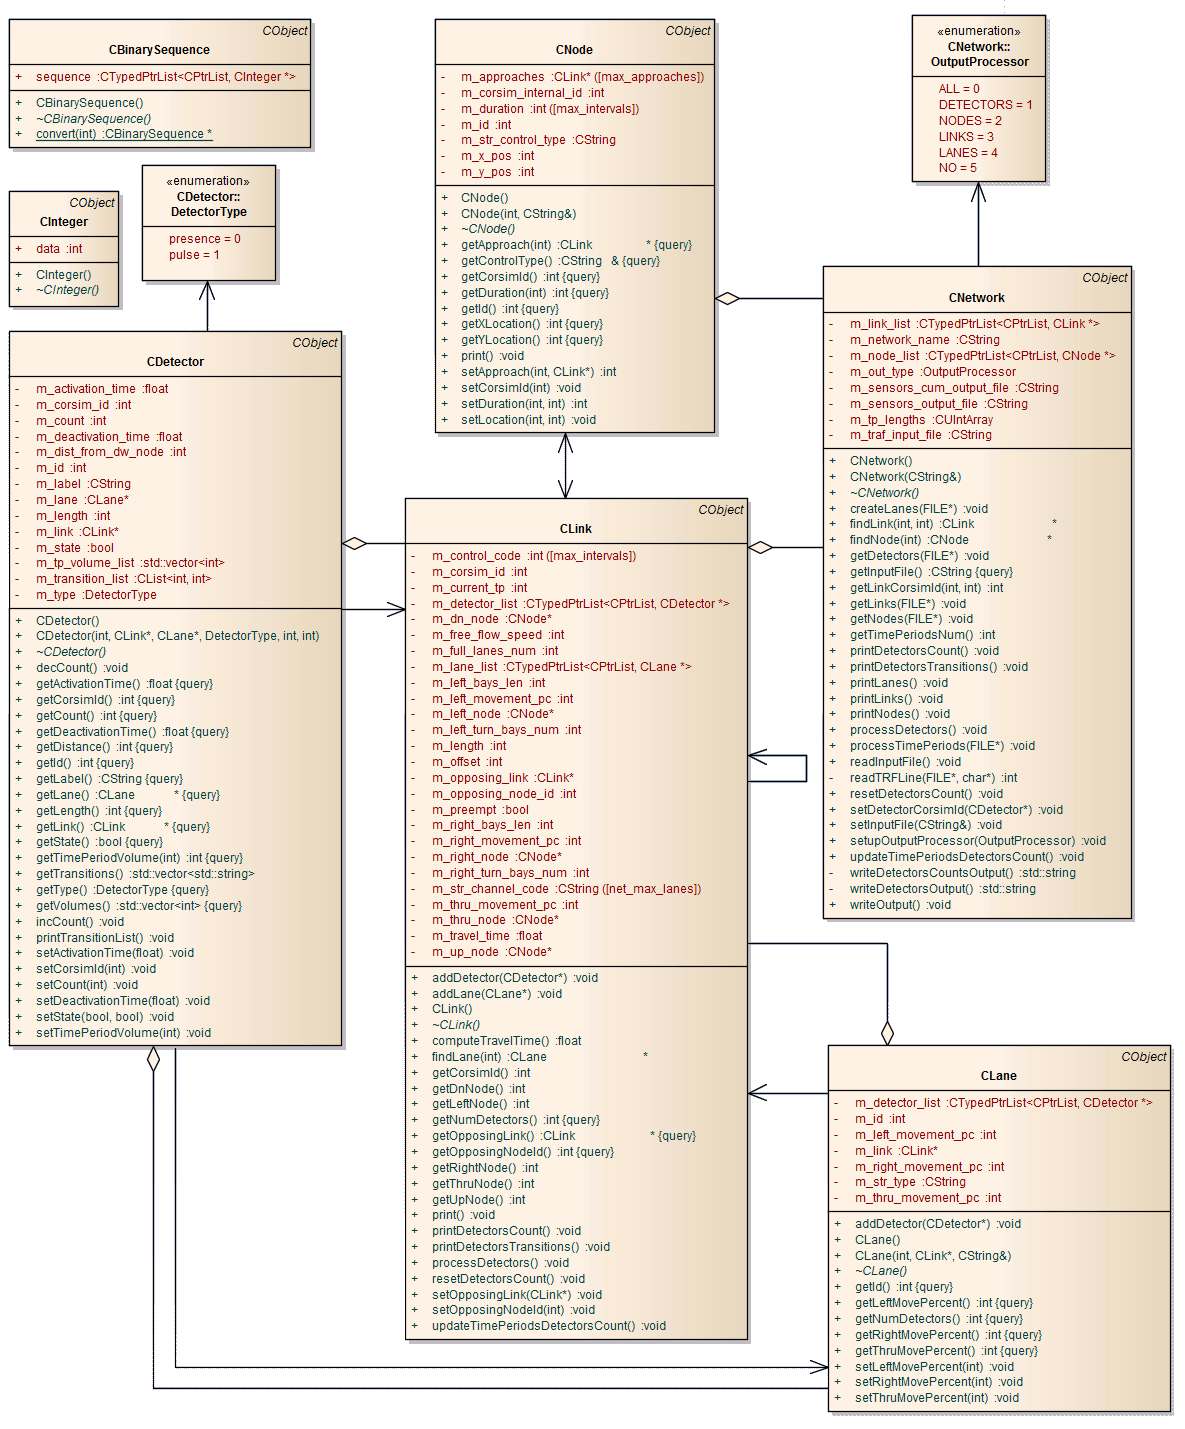
\includegraphics[width=1.4\textwidth,center]{sensors-class-diagram}
\caption[Diagramma delle classi di \acsfont{Sensors} \acs{DLL}]{Diagramma delle classi di \acsfont{Sensors} \acs{DLL}.}
\label{fig:sensors-class-diagram}
\end{figure}

\subsection{Formato dell'output}\label{subsec:sensors-dll-output}
Di seguito si presenta un esempio di file \acs{CSV} di output generato da \acsfont{Sensors} \acs{DLL}.

\lstinputsourcecode[language=pseudo, numbers=none, caption=Formato di output di \acsfont{Sensors} \acs{DLL}, label=lst:sensors-out-format]{codes/sensorsoutformat.txt}

La~\vref{tab:sensors-output-semantic} chiarisce il significato di ogni colonna dei dati tabulari restituiti da \acsfont{Sensors} \acs{DLL}.
\begin{table}[H]%
\begin{tabularx}{\columnwidth}{+l^X}
\toprule\rowstyle{\bfseries}%
Nome colonna            & Descrizione                                                                       \\
\otoprule%
time                    & Tempo di simulazione a cui è stato effettuato il monitoraggio dei sensori.        \\
tp                      & Indice del corrente periodo temporale (\ie{} \emph{time period}).                \\
identificatore sensore  & $1$ in caso di presenza di un veicolo sul rispettivo sensore, $0$ altrimenti.    \\\bottomrule
\end{tabularx}
\caption[Semantica dell'output di \acsfont{Sensors} \acs{DLL}]{Descrizione della semantica dei file \acs{CSV} generati da \acsfont{Sensors} \acs{DLL}.}
\label{tab:sensors-output-semantic}
\end{table}

Si osservi che, il fatto che il sensore \lstinline[]|D232|, in corrispondenza dell'istante $1.6$ ($5$\textsuperscript{a} colonna) abbia valore $1$ non indica che il veicolo sia stato rilevato esattamente in tale istante, bensì ciò indica che durante l'intervallo temporale $[\,1.5,1.6\,]$ tale sensore è stato attivato dal passaggio di un veicolo.

\section{Applicativi di supporto}\label{sec:dataset-tools}
Al fine di automatizzare e facilitare la creazione di dataset relativi al traffico tramite la \acs{RTE} trattata nel corrente capitolo, si è sviluppato un insieme di strumenti dediti alla manipolazione dei file di output di \acsfont{Sensors} \acs{DLL}.

Di seguito si elencano le operazioni di manipolazione che tali strumenti supportano:
\begin{enumerate}
    \item sostituzione (e eventualmente rimozione) della colonna relativa ai periodi temporali con una nuova colonna che rappresenti la classe di un insieme di osservazioni; tale colonna è automaticamente generata in base a un sistema di regole (\eg{} \emph{matching} tra periodo temporale e classe).
    \item partizionamento del file di output di \acsfont{Sensors} \acs{DLL} in più file in base a vincoli temporali (\eg{} divisione del file in blocchi di $60$ secondi ciascuno)
    \item ottimizzazione del file tramite rimozione delle linee duplicate (\ie{} linee in cui non è avvenuto alcun cambiamento di stato dei sensori).
\end{enumerate}
